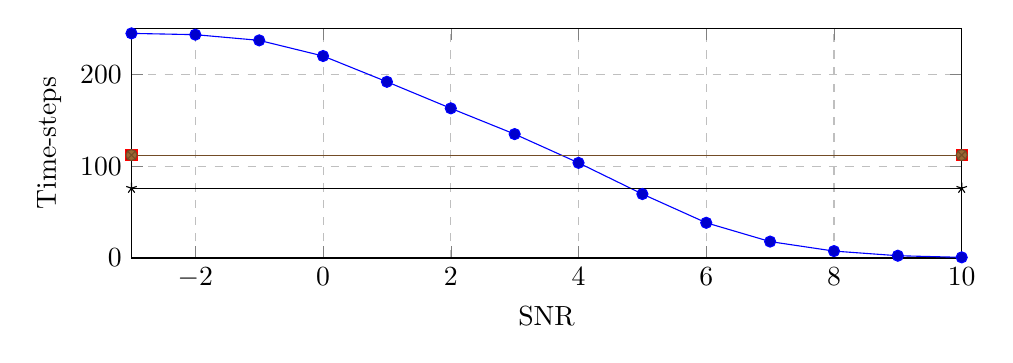
\begin{tikzpicture}

\begin{axis}[
scale=1,
xmin=-3,
xmax=10,
ymin=0,
ymax=250,
ymajorgrids=true,
xmajorgrids=true,
grid style=dashed,
width=\linewidth, height=4.5cm,
xlabel={SNR},
ylabel={Time-steps},
%ylabel shift=-7,
legend cell align={left},
legend pos=north east,
legend style={
	column sep=0mm,
	font=\fontsize{9pt}{9}\selectfont,
},
legend to name=legend-RMLatcomp,
legend columns=4,
]

%\addplot
%table {
%-3 96.74
%-2 95.27
%-1 91.81
%0 85.23
%1 75.11
%2 62.16
%3 48.16
%4 34.86
%5 23.24
%6 14.11
%7 7.77
%8 3.57
%9 1.37
%10 0.42
%};
%\addlegendentry{GA}

\addplot
table {
-3 244.39
-2 242.99
-1 236.79
0  219.77
1  191.72
2  162.85
3  134.82
4  103.53
5  69.610
6  38.330
7  17.890
8  7.5500
9  2.5100
10 0.7300
};
\addlegendentry{Proposed}

\addplot
table {
-3 112
10 112
};
\addlegendentry{SCL \cite{hashemi2016fast}}

\addplot
table {
-3 112
10 112
};
\addlegendentry{SCL \cite{hashemi2017fast}}

\addplot
table {
-3 76
10 76
};
\addlegendentry{SCL \cite{hanif2018fast}}

\end{axis}
\end{tikzpicture}